\hypertarget{TestStatistic_8h}{
\section{Test\-Statistic.h File Reference}
\label{TestStatistic_8h}\index{TestStatistic.h@{TestStatistic.h}}
}


This graph shows which files directly or indirectly include this file:\begin{figure}[H]
\begin{center}
\leavevmode
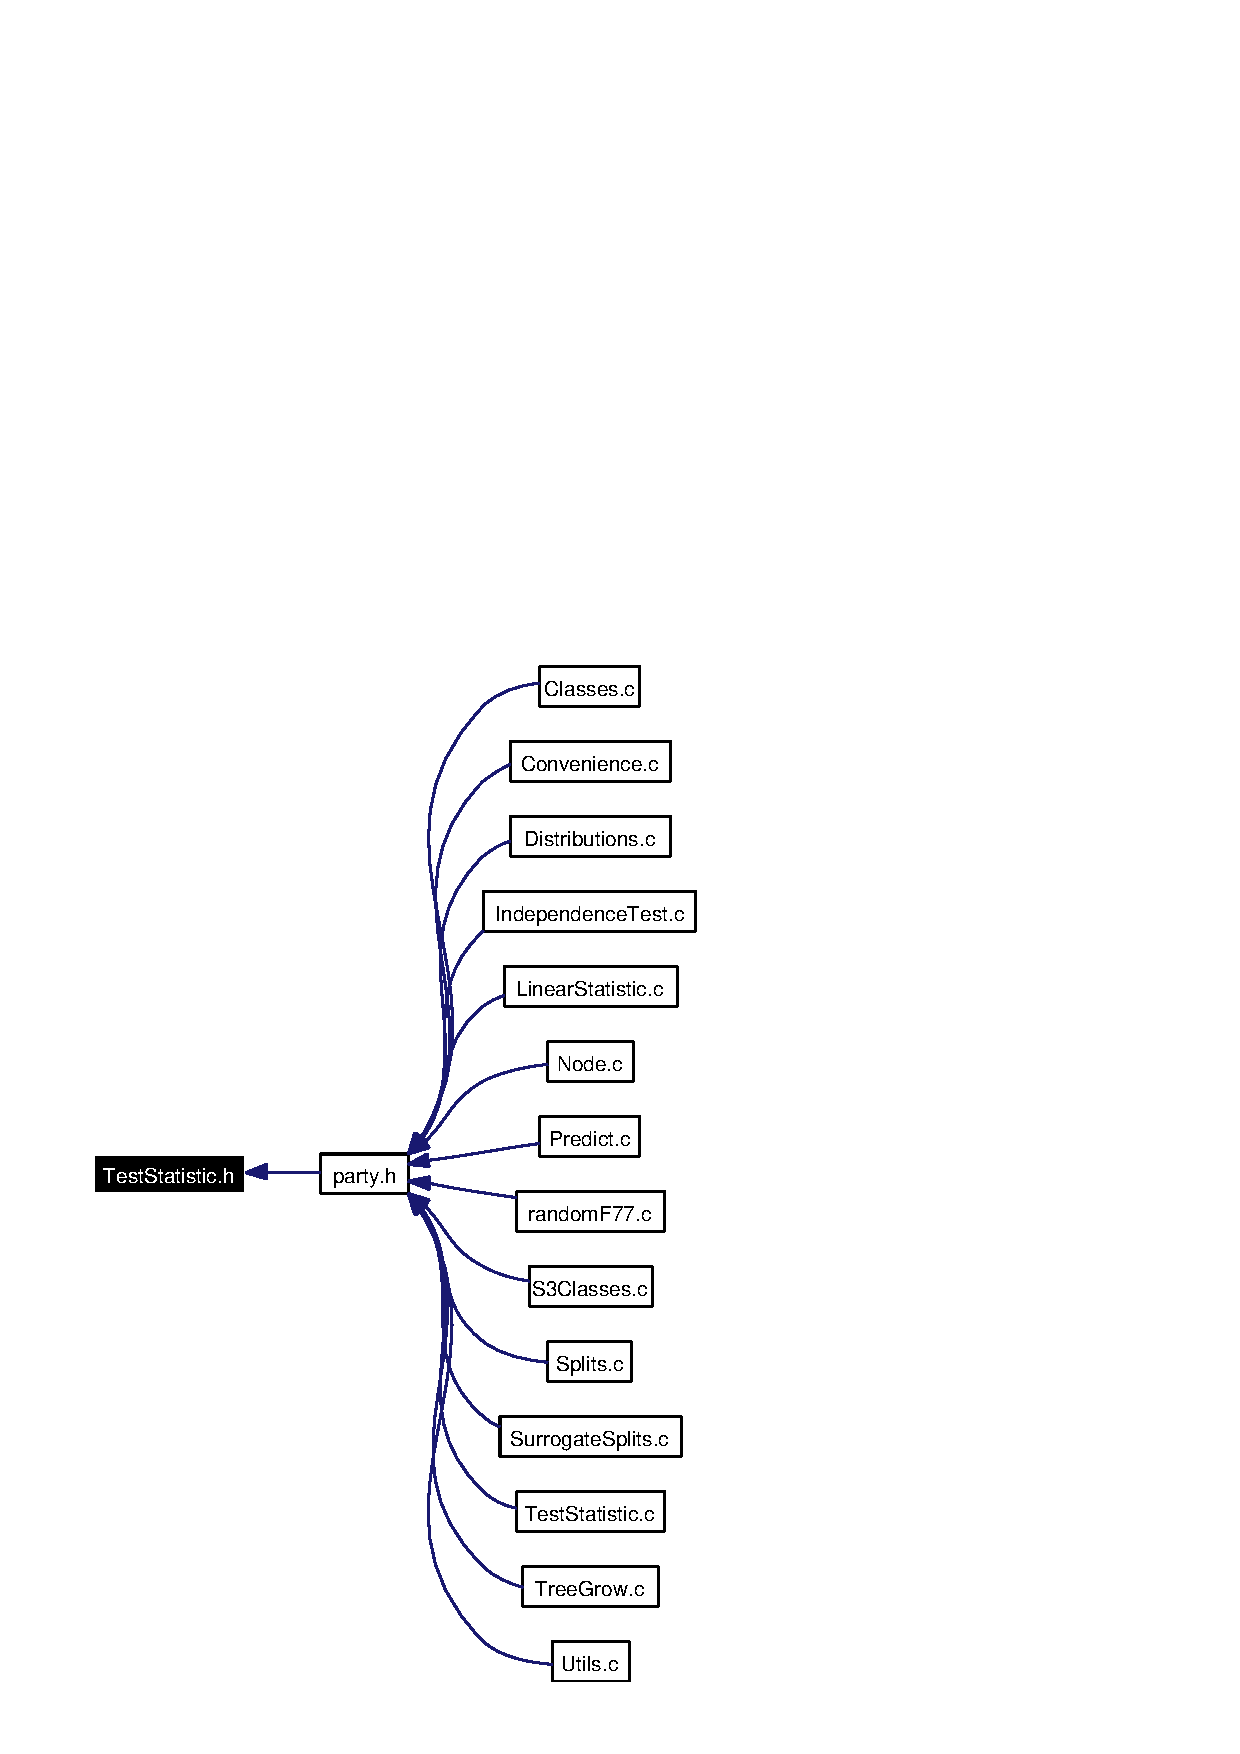
\includegraphics[width=171pt]{TestStatistic_8h__dep__incl}
\end{center}
\end{figure}
\subsection*{Functions}
\begin{CompactItemize}
\item 
void \hyperlink{TestStatistic_8h_a0}{C\_\-standardize} (const double $\ast$t, const double $\ast$mu, const double $\ast$Sigma, int pq, double tol, double $\ast$ans)
\item 
double \hyperlink{TestStatistic_8h_a1}{C\_\-maxabs\-Test\-Statistic} (const double $\ast$t, const double $\ast$mu, const double $\ast$Sigma, int pq, double tol)
\item 
double \hyperlink{TestStatistic_8h_a2}{C\_\-quadform\-Test\-Statistic} (const double $\ast$t, const double $\ast$mu, const double $\ast$Sigma\-Plus, int pq)
\end{CompactItemize}


\subsection{Function Documentation}
\hypertarget{TestStatistic_8h_a1}{
\index{TestStatistic.h@{Test\-Statistic.h}!C_maxabsTestStatistic@{C\_\-maxabsTestStatistic}}
\index{C_maxabsTestStatistic@{C\_\-maxabsTestStatistic}!TestStatistic.h@{Test\-Statistic.h}}
\subsubsection[C\_\-maxabsTestStatistic]{\setlength{\rightskip}{0pt plus 5cm}double C\_\-maxabs\-Test\-Statistic (const double $\ast$ {\em t}, const double $\ast$ {\em mu}, const double $\ast$ {\em Sigma}, int {\em pq}, double {\em tol})}}
\label{TestStatistic_8h_a1}


Maximum absolute values of standardized statistics \begin{Desc}
\item[Parameters:]
\begin{description}
\item[{\em t}]the vector of statistics \item[{\em mu}]expectations \item[{\em Sigma}]covariance matrix \item[{\em pq}]dimension of t \item[{\em tol}]tolerance for variances\end{description}
\end{Desc}


Definition at line 66 of file Test\-Statistic.c.

References C\_\-absstandardize(), and C\_\-max().

Referenced by C\_\-Test\-Statistic(), and R\_\-maxabs\-Test\-Statistic().

Here is the call graph for this function:\begin{figure}[H]
\begin{center}
\leavevmode
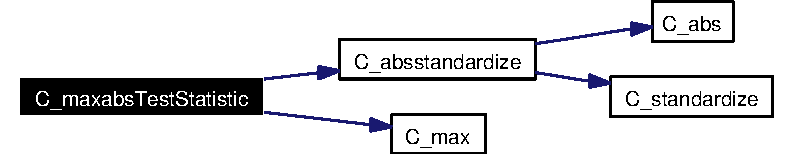
\includegraphics[width=203pt]{TestStatistic_8h_a1_cgraph}
\end{center}
\end{figure}
\hypertarget{TestStatistic_8h_a2}{
\index{TestStatistic.h@{Test\-Statistic.h}!C_quadformTestStatistic@{C\_\-quadformTestStatistic}}
\index{C_quadformTestStatistic@{C\_\-quadformTestStatistic}!TestStatistic.h@{Test\-Statistic.h}}
\subsubsection[C\_\-quadformTestStatistic]{\setlength{\rightskip}{0pt plus 5cm}double C\_\-quadform\-Test\-Statistic (const double $\ast$ {\em t}, const double $\ast$ {\em mu}, const double $\ast$ {\em Sigma\-Plus}, int {\em pq})}}
\label{TestStatistic_8h_a2}


Quadratic form t(t - mu) Sigma\-Plus (t - mu) \par
 \begin{Desc}
\item[Parameters:]
\begin{description}
\item[{\em t}]the vector of statistics \item[{\em mu}]expectations \item[{\em Sigma\-Plus}]Moore-Penrose inverse \item[{\em pq}]dimension of t\end{description}
\end{Desc}


Definition at line 110 of file Test\-Statistic.c.

Referenced by C\_\-Test\-Statistic(), and R\_\-quadform\-Test\-Statistic().\hypertarget{TestStatistic_8h_a0}{
\index{TestStatistic.h@{Test\-Statistic.h}!C_standardize@{C\_\-standardize}}
\index{C_standardize@{C\_\-standardize}!TestStatistic.h@{Test\-Statistic.h}}
\subsubsection[C\_\-standardize]{\setlength{\rightskip}{0pt plus 5cm}void C\_\-standardize (const double $\ast$ {\em t}, const double $\ast$ {\em mu}, const double $\ast$ {\em Sigma}, int {\em pq}, double {\em tol}, double $\ast$ {\em ans})}}
\label{TestStatistic_8h_a0}


Standardizes a statistic t of length pq with mean mu and covariance Sigma for variances $>$ tol \par
 \begin{Desc}
\item[Parameters:]
\begin{description}
\item[{\em t}]the vector of statistics \item[{\em mu}]expectations \item[{\em Sigma}]covariance matrix \item[{\em pq}]dimension of t \item[{\em tol}]tolerance for variances \item[{\em ans}]return value; a pointer to a REALSXP-vector of length pq\end{description}
\end{Desc}


Definition at line 23 of file Test\-Statistic.c.

Referenced by C\_\-absstandardize(), C\_\-Node(), and R\_\-splitcategorical().